\subsection{ออกแบบแบบจำลองของหุ่นยนต์ฮิวมานอยด์ UTHAI}

\begin{figure}[!ht]
	\centering
	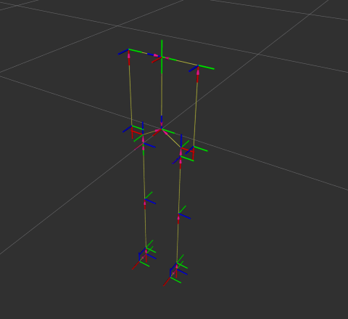
\includegraphics[width=\textwidth]{chapter4/images/urdf_rviz0.png}
	\caption{URDF ที่มีแต่โครงไม่มีก้านต่อ}
\end{figure}
\begin{figure}[!ht]
    \centering
    \begin{subfigure}[b]{0.29\textwidth}
        \centering
        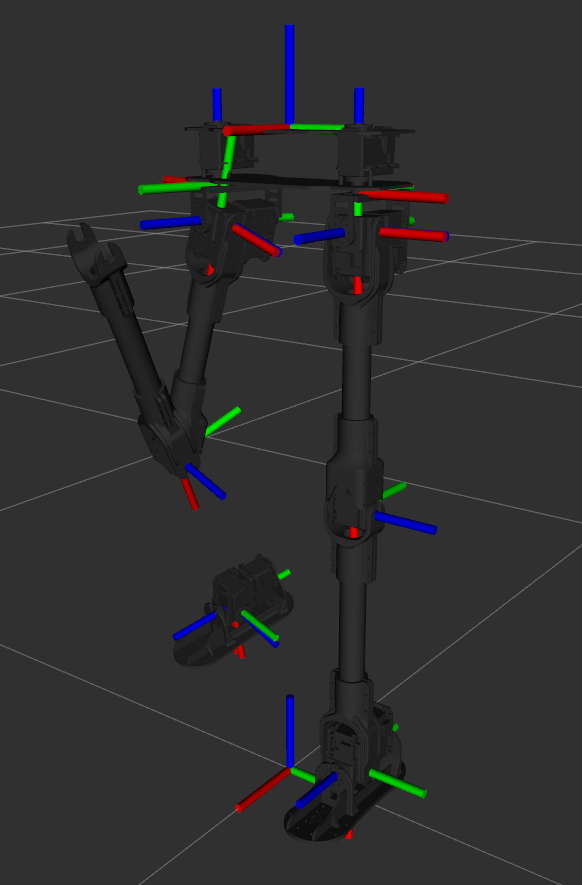
\includegraphics[width=\textwidth]{chapter4/images/urdf_rviz1.png}
        \caption{URDF ที่เกิดข้อผิดพลาด}
    \end{subfigure}
    \hfill
    \begin{subfigure}[b]{0.65\textwidth}
        \centering
        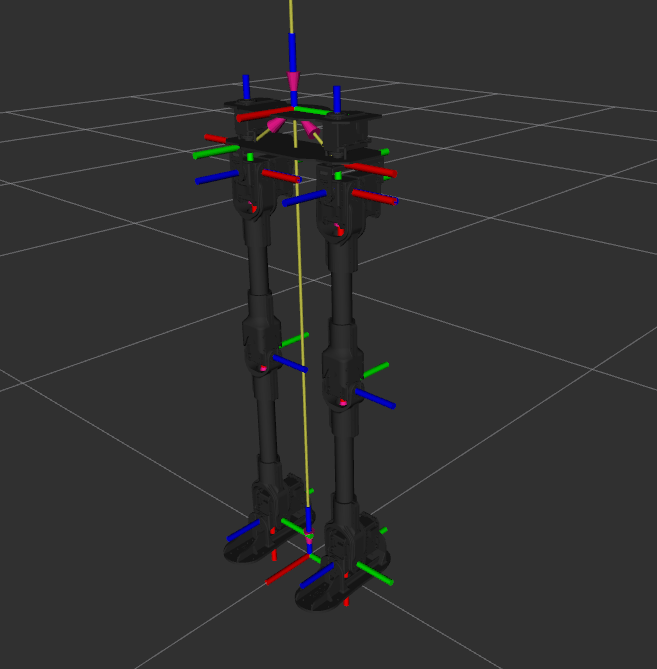
\includegraphics[width=\textwidth]{chapter4/images/urdf_rviz2.png}
        \caption{URDF ที่ทำงานได้ถูกต้อง}
    \end{subfigure}
    \caption{URDF ที่แสดงผลใน RViz}
\end{figure}

\subsection{การสั่งงานข้อต่อใน RViz ผ่าน GUI}
หลังจากที่ทำการทดลองเสร็จแล้วพบว่าสิ่งที่ขาดหายไปคือการตั้งค่า Joint limit ให้กับหุ่นยนต์ฮิวมานอยด์ในโปรแกรม RViz
จึงต้องกลับไปแก้ค่าและทดสอบใหม่ จากนั้นถือว่าการทดลองเสร็จสิ้น สามารถที่จะควบคุมการเคลื่อนไหวของแต่ละข้อต่อผ่าน GUI ได้

\begin{figure}[!ht]
    \centering
    \begin{subfigure}[b]{0.29\textwidth}
        \centering
        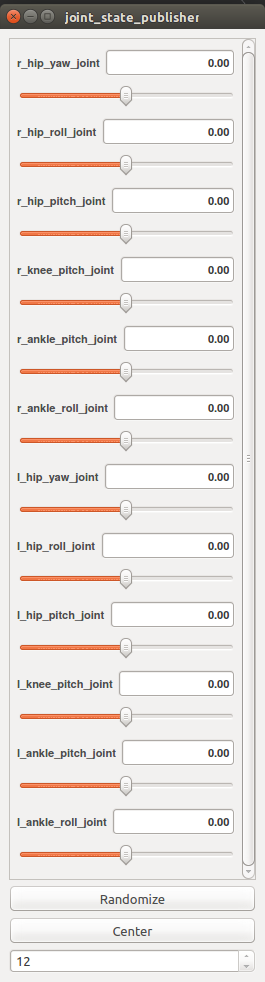
\includegraphics[width=\textwidth]{chapter4/images/uthai_rviz_gui.png}
        \caption{GUI สำหรับสั่งงานแต่ละข้อต่อ}
    \end{subfigure}
    \hfill
    \begin{subfigure}[b]{0.65\textwidth}
        \centering
        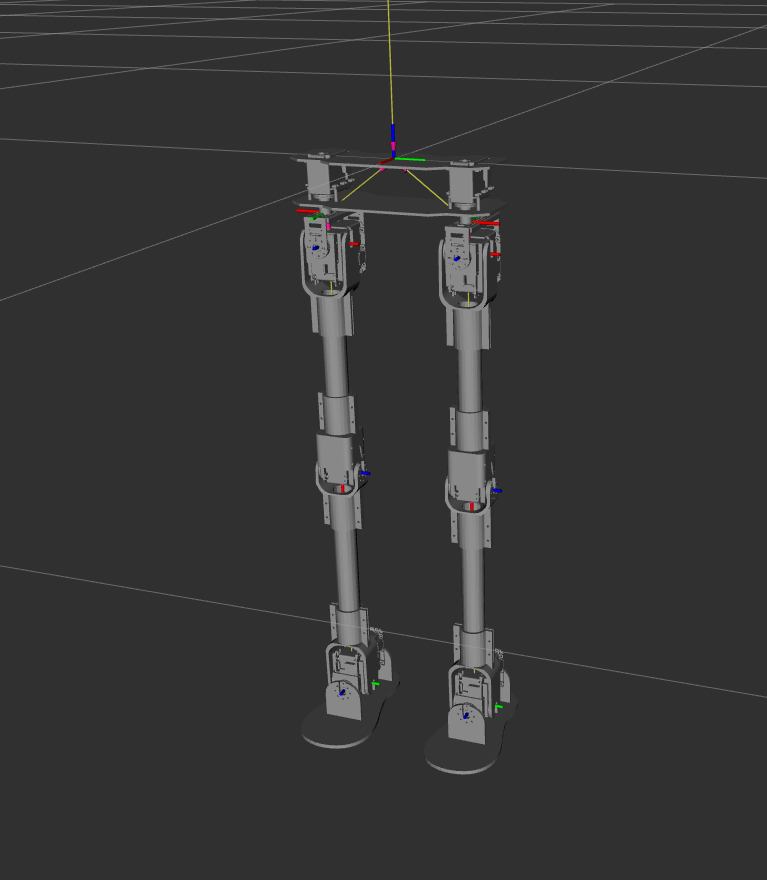
\includegraphics[width=\textwidth]{chapter4/images/uthai_rviz_model.png}
        \caption{หุ่นยนต์ที่แสดงผลในโปรแกรม RViz}
    \end{subfigure}
    \caption{การสั่งการข้อต่อใน RViz ผ่าน GUI}
\end{figure}




\clearpage
\subsection{รับค่าจากมอเตอร์แล้วมาแสดงผลใน RViz}

\begin{figure}[!ht]
    \centering
    \begin{subfigure}[b]{0.45\textwidth}
        \centering
        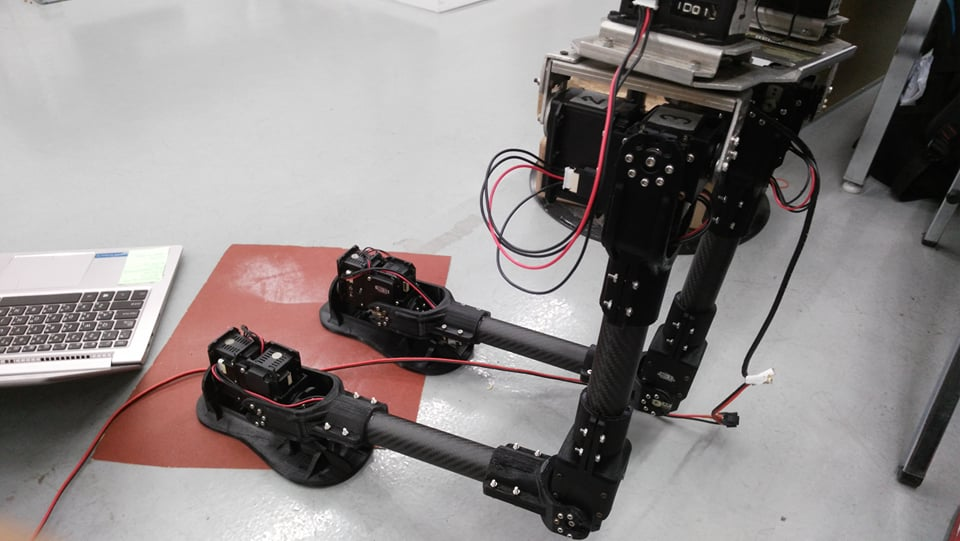
\includegraphics[width=\textwidth]{chapter4/images/robot_2_rviz1.jpg}
        \caption{หุ่นยนต์ตัวจริง}
    \end{subfigure}
    \hfill
    \begin{subfigure}[b]{0.45\textwidth}
        \centering
        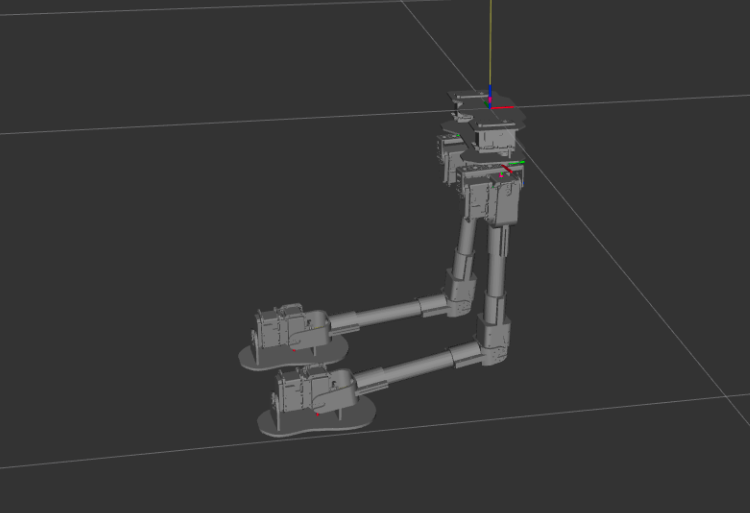
\includegraphics[width=\textwidth]{chapter4/images/robot_2_rviz1.png}
        \caption{หุ่นยนต์ใน RViz}
    \end{subfigure}
    \caption{การแสดงผลท่าทาง 1}
	\label{fig:robot_2_rviz1}
\end{figure}

\begin{figure}[!ht]
    \centering
    \begin{subfigure}[b]{0.45\textwidth}
        \centering
        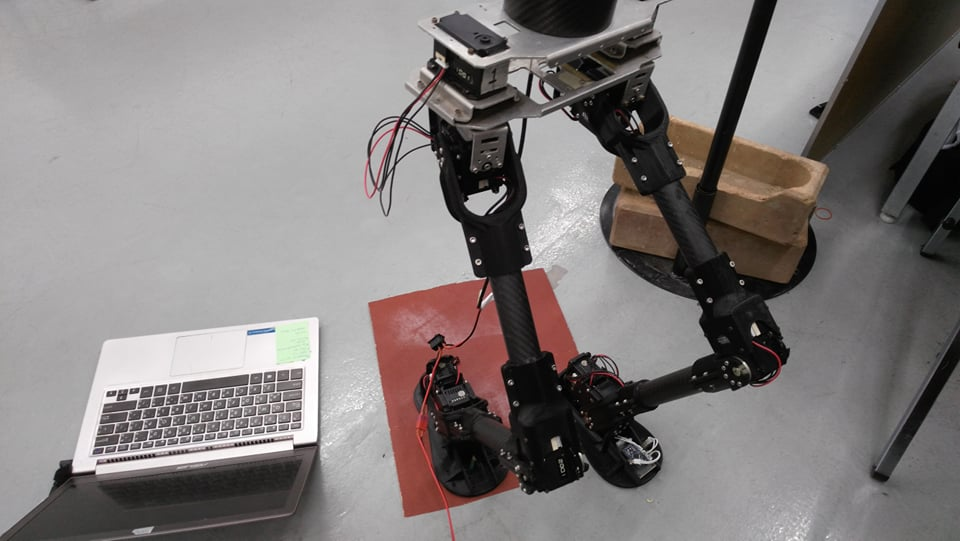
\includegraphics[width=\textwidth]{chapter4/images/robot_2_rviz2.jpg}
        \caption{หุ่นยนต์ตัวจริง}
    \end{subfigure}
    \hfill
    \begin{subfigure}[b]{0.35\textwidth}
        \centering
        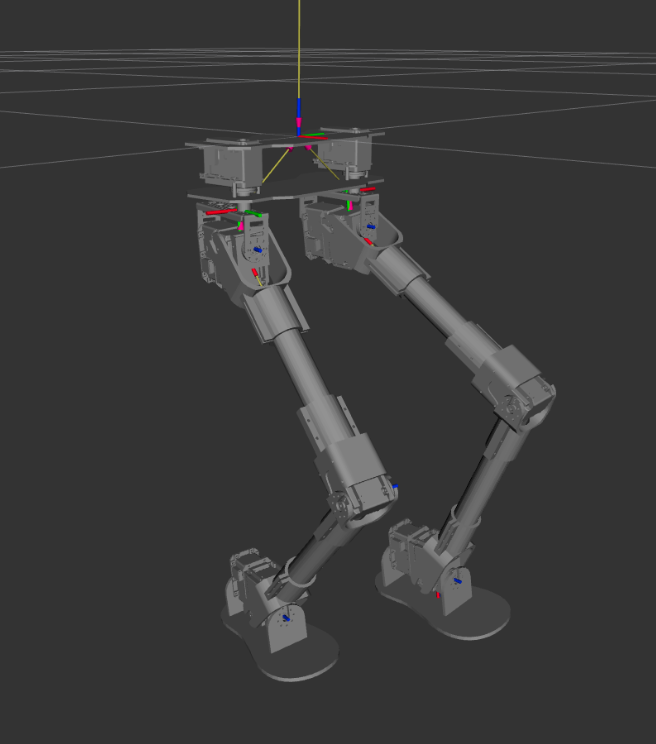
\includegraphics[width=\textwidth]{chapter4/images/robot_2_rviz2.png}
        \caption{หุ่นยนต์ใน RViz}
    \end{subfigure}
    \caption{การแสดงผลท่าทาง 2}
	\label{fig:robot_2_rviz2}
\end{figure}

\begin{figure}[!ht]
    \centering
    \begin{subfigure}[b]{0.45\textwidth}
        \centering
        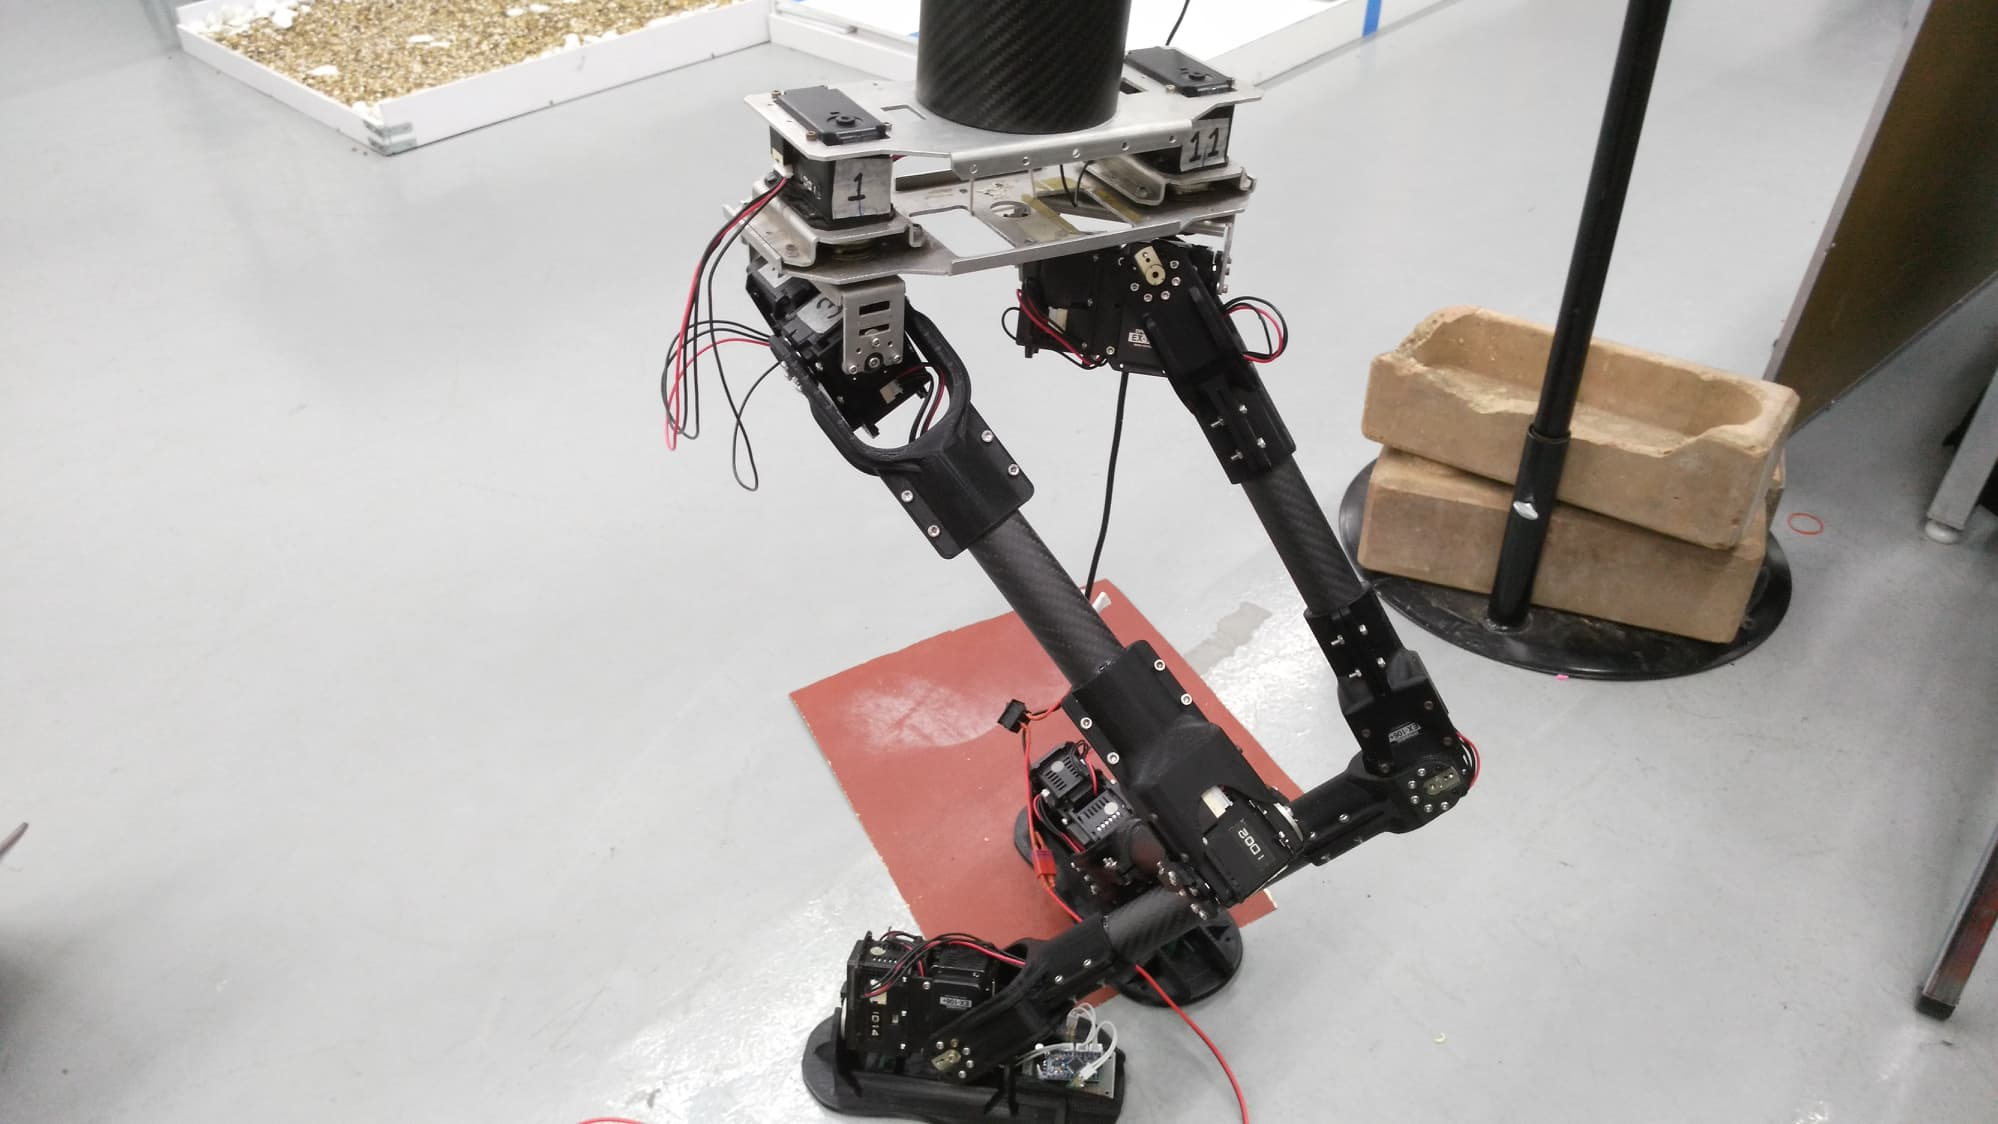
\includegraphics[width=\textwidth]{chapter4/images/robot_2_rviz3.jpg}
        \caption{หุ่นยนต์ตัวจริง}
    \end{subfigure}
    \hfill
    \begin{subfigure}[b]{0.35\textwidth}
        \centering
        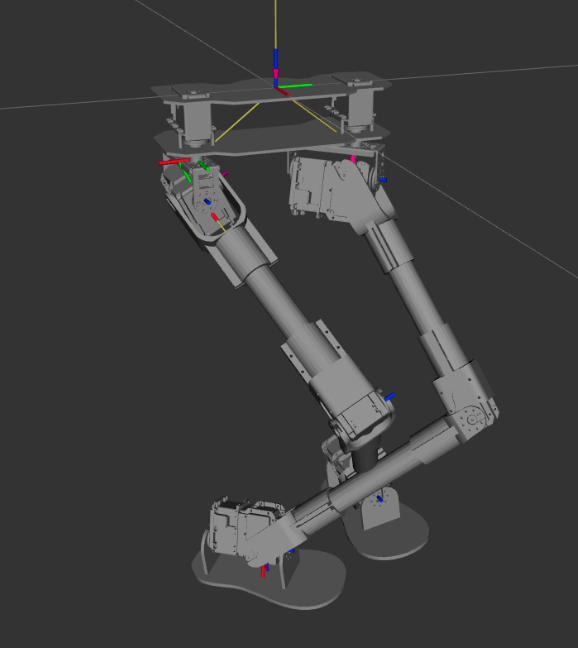
\includegraphics[width=\textwidth]{chapter4/images/robot_2_rviz3.png}
        \caption{หุ่นยนต์ใน RViz}
    \end{subfigure}
    \caption{การแสดงผลท่าทาง 3}
	\label{fig:robot_2_rviz3}
\end{figure}



\clearpage
\subsection{รับค่าจุดศูนย์กลางมวลจาก MATLAB แล้วมาแสดงผลใน RViz}

\begin{figure}[!ht]
	\centering
	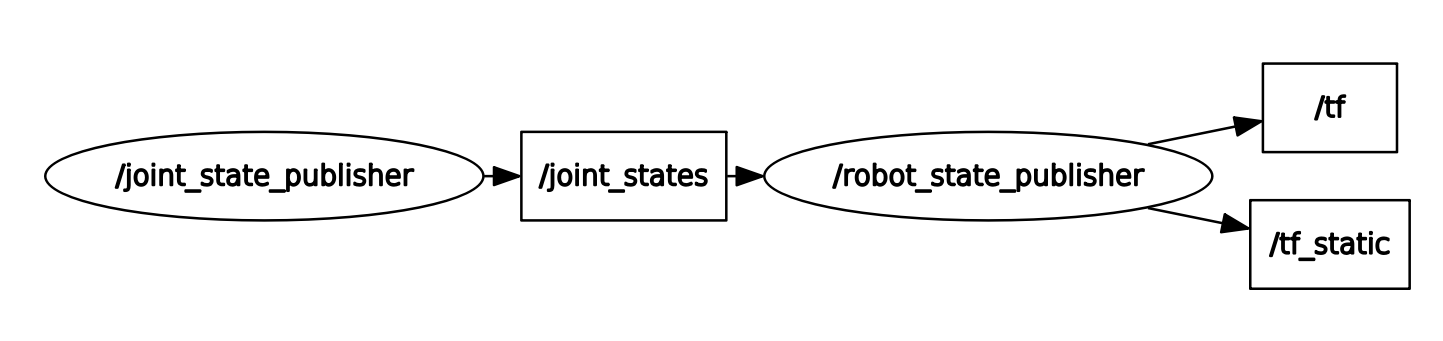
\includegraphics[width=\textwidth]{chapter4/images/com_uthai_node0.png}
	\caption{การเชื่อมต่อกันระหว่าง Node ก่อนเชื่อมต่อเซอร์โวมอเตอร์}
\end{figure}
\begin{figure}[!ht]
	\centering
	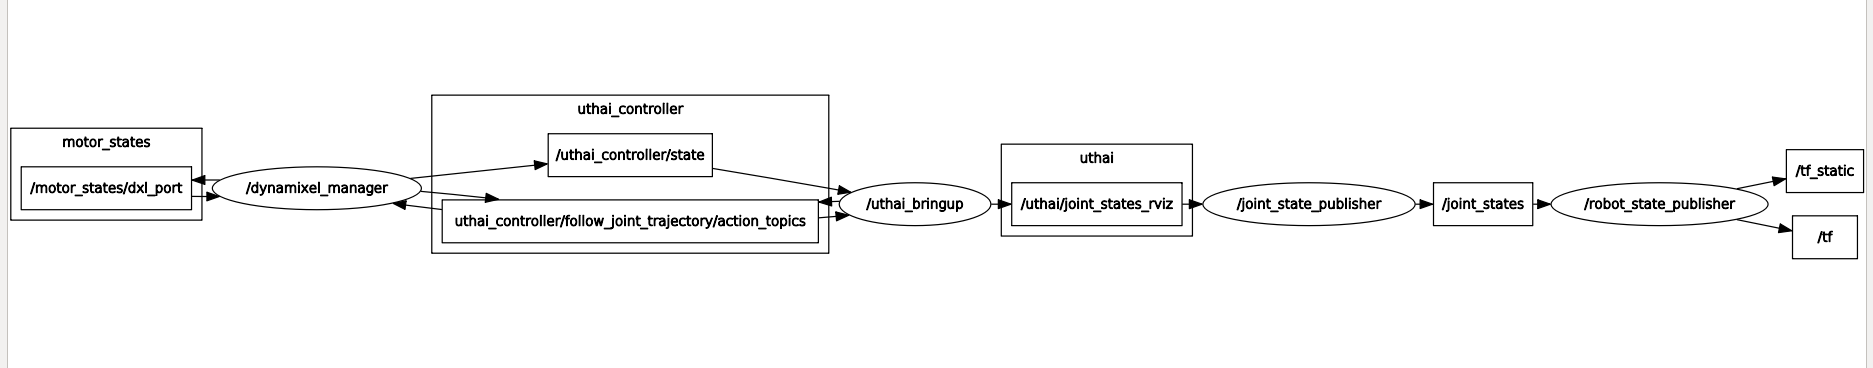
\includegraphics[width=\textwidth]{chapter4/images/com_uthai_node.png}
	\caption{การเชื่อมต่อกันระหว่าง Node หลังเชื่อมต่อเซอร์โวมอเตอร์}
\end{figure}
\begin{figure}[!ht]
	\centering
	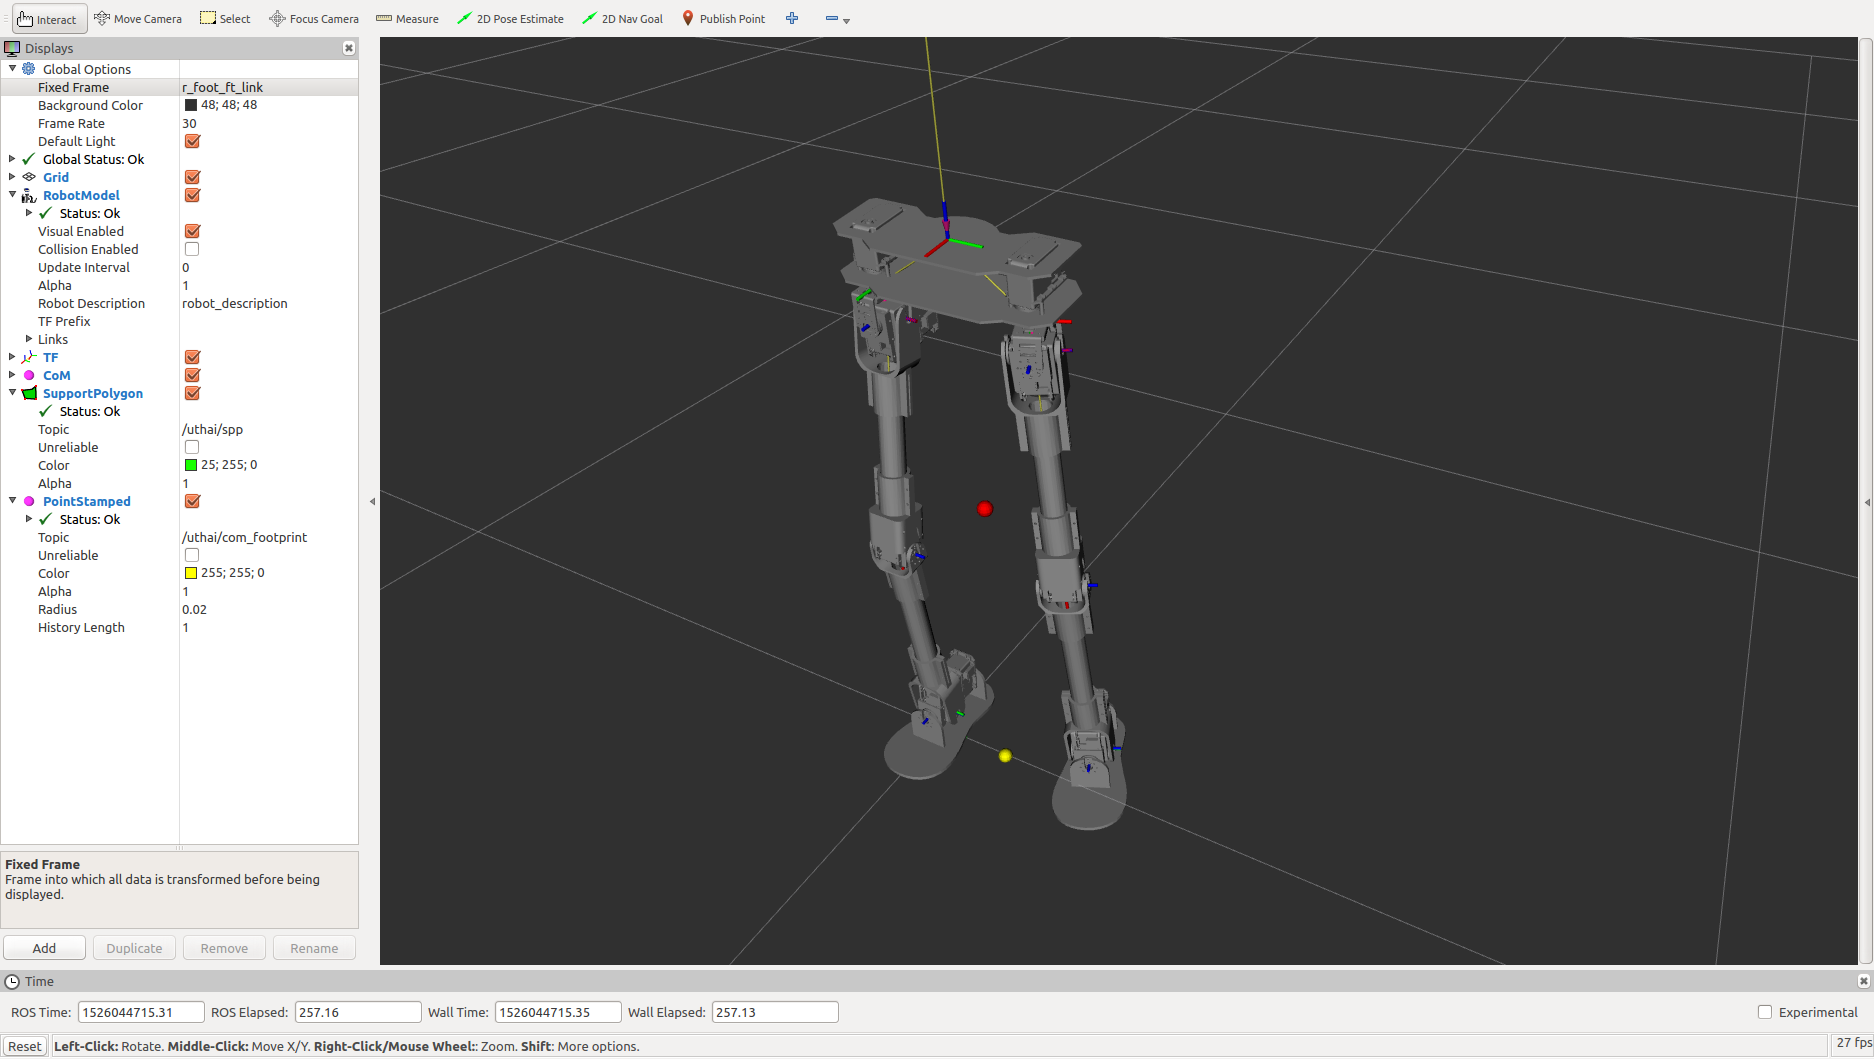
\includegraphics[width=\textwidth]{chapter4/images/com_uthai.png}
	\caption{การประมวลผลตำแหน่งหาจุดศูนย์กลางด้วย MATLAB}
\end{figure}
